\documentclass[10pt]{beamer}
\usetheme{Antibes}

\usepackage[utf8]{inputenc}
\usepackage{amsmath}
\usepackage{amsfonts}
\usepackage{amssymb}
\usepackage{graphicx}
\usepackage{algorithm,algorithmic}
\usepackage{animate}
\usepackage{booktabs}
\usepackage{subcaption}
\usepackage{minted}
\usepackage{hyperref}
\usepackage{xcolor}


\DeclareMathOperator*{\argmax}{arg\,max}
\DeclareMathOperator*{\argmin}{arg\,min}



\author{José Jiménez}
\title{Bayesian Optimization in Machine Learning}

\titlegraphic{

	
\includegraphics[scale=0.15]{figures/UPC-logo.jpg} \hfill
	
\includegraphics[scale=0.63]{figures/logo_home_nou.png}

	}

\institute{Master's Thesis \vfill Master's degree in Statistics and Operations Research}

\date{\tiny supervised by Josep Ginebra\textsuperscript{1}\vfill
	\textsuperscript{1} Department of Statistics and Operations Research. ETSEIB.}

\subject{Bayesian Optimization}

\setbeamercovered{transparent}

\setbeamertemplate{theorems}[ams style] 


\begin{document}
	\maketitle
	
	\begin{frame}
		\frametitle{Goals of this thesis}
		This Master's thesis has different and complimentary aims:
		
		\begin{itemize}
			\item Provide an introduction to both Gaussian Process regression and Bayesian optimization. 
			\item Show that the Bayesian Optimization framework works in several real-world machine learning tasks.
			\item Write a complete software package (pyGPGO) for users to apply Bayesian Optimization in their research.
		\end{itemize}
	\end{frame}
	
	\begin{frame}
		\frametitle{Organization of the work}
		Organized in 4 self-contained chapters.
		\begin{itemize}
			\item \textbf{Chapter 2} focuses on an introduction to regression problems using Gaussian Processes. These are surrogate models we will use for Bayesian Optimization.
			\item \textbf{Chapter 3} covers the main topic in this work, Bayesian Optimization.
			\item \textbf{Chapter 4} presents experiments using the Bayesian Optimization framework. Mostly mid-sized supervised-learning problems.
			\item \textbf{Chapter 5} provides technical explanations for pyGPGO, the software developed alongside this manual.
		\end{itemize}
	\end{frame}
	
	\begin{frame}
		\frametitle{A brief introduction}
		Overall, Bayesian Optimization focuses on:
		
		\begin{equation}
			\max_{\boldsymbol{x}\in \mathcal{A}} f(x)
		\end{equation}
		
		We make almost no assumptions about $f$:
		\begin{itemize}
			\item $f$ may not have a closed-form expression.
			\item Evaluations of $f$ may be noisy.
			\item No gradient information needed.
		\end{itemize}
		
		An example arises when optimizing the \textit{loss} function of a machine-learning model, depending on its hyperparameters (e.g. log-loss):
		
		\begin{equation}
		\mathcal{L}(\boldsymbol{y}, \boldsymbol{\hat{y}}) = -\dfrac{1}{n} \sum_i \left(y_i \log(\hat{y_i}) + (1 - y_i)\log(1-\hat{y_i})\right)
		\end{equation}

	\end{frame}
	
	\begin{frame}
		\frametitle{Gaussian Process Regression: basic definitions}
		\begin{definition}
			A Gaussian Process is a collection of random variables, any finite number of which have a joint Gaussian distribution. This process is defined by two functions. Its \textit{mean function}:
			
			\begin{equation}
m(\boldsymbol{x}) = \mathbb{E}\left[f(\boldsymbol{x})\right]
			\end{equation}
			
			and its \textit{covariance function}:
			
			\begin{equation}
			k(\boldsymbol{x}, \boldsymbol{x'}) = \mathbb{E}\left[\left( f(\boldsymbol{x}) - m(\boldsymbol{x}) \right)\left( f(\boldsymbol{x}') - m(\boldsymbol{x}')\right)\right]
			\end{equation}
			
			We say that $f$ is a Gaussian Process with mean $m(\boldsymbol{x})$ and covariance function $k(\boldsymbol{x}, \boldsymbol{x}')$ and write:
			
			\begin{equation}
			f(\boldsymbol{x}) \sim \mathcal{GP}\left(m(\boldsymbol{x}), k(\boldsymbol{x}, \boldsymbol{x'}) \right)
			\end{equation}
			
			\end{definition}
		\end{frame}
			
		\begin{frame}	
			\frametitle{Gaussian Process Regression: basic definitions}
			Define then a covariance function, such as the \textit{squared exponential} kernel:
			
			\begin{equation}
			k(\boldsymbol{x}, \boldsymbol{x}') = \exp\left(-\dfrac{1}{2}|\boldsymbol{x} - \boldsymbol{x}'|^2\right)
			\end{equation}
			
			where $|.|$ denotes the standard $L_2$ norm. Drawing samples from a Gaussian Process, assuming zero mean, for given finite inputs $X_*$ simplifies to sampling from:
			
			\begin{equation}
			\label{fprior}
			\boldsymbol{f_*} \sim \mathcal{N}\left(\boldsymbol{0}, K(X_*, X_*)\right)
			\end{equation}
			
		\end{frame}
		
		\begin{frame}
			\frametitle{Gaussian Process Regression: prediction}
			Assume training data  $\mathcal{D} = \left\lbrace \left(\boldsymbol{x_i}, y_i\right) | i = 1,\dots,n\right\rbrace$
			\begin{block}{Prediction using GP prior}
				Let $\boldsymbol{y}$ and $\boldsymbol{f_*}$ be jointly Gaussian:
				
				\begin{equation}
				\begin{bmatrix}
				\boldsymbol{y}\\
				\boldsymbol{f_*}
				\end{bmatrix} \sim \mathcal{N}\left(
				\boldsymbol{0},
				\begin{bmatrix}
				K(X, X) + \sigma^2_n I && K(X, X_*) \\
				K(X_*, X) && K(X_*, X_*)
				\end{bmatrix}
				\right)
				\end{equation}
				
				We want to condition $\boldsymbol{f_*}$ over $\boldsymbol{y}$.
				
				\begin{equation}
				\boldsymbol{f_*|y} \sim \mathcal{N}(\boldsymbol{\overline{f_*}},  Cov(\boldsymbol{f_*}))
				\end{equation}
				
				where:
				
				\begin{align}
				\begin{split}
				\boldsymbol{\overline{f_*}} &= K(X_*, X)\left(K(X, X) + \sigma^2_n I   \right)^{-1}\boldsymbol{y}\\
				Cov(\boldsymbol{f_*}) &= K(X_*, X_*) - K(X_*, X)\left(K(X, X) + \sigma_n^2 I \right)^{-1}K(X, X_*)
				\end{split}
				\end{align}
				
			
			\end{block}
		\end{frame}
		
		\begin{frame}
			\frametitle{Gaussian Process Regression: an example}
			\begin{figure}
				\includegraphics[width=\textwidth]{../figures/chapter2/GPsine}
			\end{figure}
		\end{frame}
		
		\begin{frame}
			\frametitle{Gaussian Process Regression: on covariance functions}

			\begin{block}{Some common covariance function choices}
				\begin{equation}
				\begin{matrix}
				k_{SE}(r) = \exp\left(-\dfrac{r^2}{2l^2} \right) && 				k_{\textrm{Matèrn}}(r) = \dfrac{2^{1-\nu}}{\Gamma(\nu)}\left(\dfrac{\sqrt{2\nu} r}{l}    \right)^\nu K_\nu\left( \dfrac{
					\sqrt{2\nu}r}{l} \right) \\
				k_{\mathrm{GE}}(r) = \exp\left( - \left(\dfrac{r}{l}\right)^\gamma  \right) && k_{RQ}(r) = \left( 1 + \dfrac{r^2}{2\alpha l^2} \right)^{-\alpha}
				\end{matrix}
				\end{equation}
				
				where $r=|\boldsymbol{x} - \boldsymbol{x'}|$. Observations are noisy:
				
				\begin{equation}
					k^y(\boldsymbol{x}_p, \boldsymbol{x}_q) = \sigma^2_f k(\boldsymbol{x}_p, \boldsymbol{x}_q) + \sigma^2_n \delta_{pq} \,
				\end{equation} 
				
			\end{block}
		\end{frame}
		
		\begin{frame}
			\frametitle{Gaussian Process Regression: Type II Maximum-Likelihood}
			An empirical Bayes approach to choosing hyperparameters. Noticing that $\boldsymbol{y} \sim \mathcal{N}(\boldsymbol{0}, K + 
			\sigma_n^2 I)$
			\begin{block}{Marginal log-likelihood}
				\begin{equation}
				\log p(\boldsymbol{y}|X) = - \dfrac{1}{2}\boldsymbol{y}^T(K + \sigma^2_n I)^{-1}\boldsymbol{y} - \dfrac{1}{2}\log |K + \sigma^2_n I| - \dfrac{n}{2}\log 2\pi
				\end{equation}
			\end{block}
			
			\begin{block}{Derivative w.r.t hyperpameters}
				\begin{equation}
				\dfrac{\partial}{\partial \theta_j}\log p(\boldsymbol{y}|X, \boldsymbol{\theta}) = \dfrac{1}{2}\boldsymbol{y}^T K^{-1}\dfrac{\partial K}{\partial \theta_j}K^{-1}\boldsymbol{y} - \dfrac{1}{2}\textrm{tr}\left(K^{-1} \dfrac{\partial K}{\partial \theta_j} \right)
				\end{equation}
			\end{block}
		\end{frame}
			
		\begin{frame}
			\frametitle{Gaussian Process Regression: incorporating diff. priors}
			We have assumed $m(\boldsymbol{x}) = 0$ for simplicity. If we dispose of prior knowledge, we can use it
			
			\begin{block}{Different prior mean}
				\begin{equation}
				f(\boldsymbol{x}) \sim \mathcal{G}\mathcal{P}\left(m(\boldsymbol{x}), k(\boldsymbol{x}, \boldsymbol{x^*})\right)
				\end{equation}
				
				Posterior mean becomes:
				
				\begin{equation}
				\boldsymbol{f}_* = \boldsymbol{m}(X_*) + k(X_*, X)K^{-1}\left(\boldsymbol{y} - \boldsymbol{m}(X)\right) 
				\end{equation}
				
				Posterior variance remains unchanged.
			\end{block}
		\end{frame}
		
		\begin{frame}
			\frametitle{Gaussian Process Regression: marginalizing over hyperparameters}
			The full Bayesian approach does not optimize the marginal likelihood, but integrates the uncertainty of hyperparameters $\theta$ into the model, either using MCMC or Variational Inference techniques.
			
			\begin{block}{Full Bayesian approach}
				\begin{equation}
				\theta \sim p_{h}(\theta)
				\end{equation}
				\begin{equation}
				\boldsymbol{f} \sim \mathcal{N}(0, \Sigma_\theta)
				\end{equation}
				\begin{equation}
				\mathcal{L(\boldsymbol{f})} = p(\mathrm{data}|\boldsymbol{f}) = p(\boldsymbol{y}|\boldsymbol{f})
				\end{equation}
				
				We wish to sample from the joint posterior under unknowns:
				
				\begin{equation}
				p(\boldsymbol{f}, \theta|\, \mathrm{data}) \propto \mathcal{L}(\boldsymbol{f})p(\boldsymbol{f}) p_h(\theta)
				\end{equation}
			\end{block}
			Several strategies for sampling from latent Gaussian models proposed in main text.	
		\end{frame}
		
		\begin{frame}
			\frametitle{Bayesian Optimization: introduction}
			Again, assume:
			 \begin{equation}
			 \max_{\boldsymbol{x}\in \mathcal{A}} f(\boldsymbol{x})
			 \end{equation}
			 
			 Assume that we have sampled our function $f$ to optimize a small number of times $n$. Providing us with training data:

			 \begin{equation}
			 \mathcal{D}_n = \left\lbrace \boldsymbol{x}_i, y_i, i=1,\dots,n\right\rbrace.
			 \end{equation}
			 
			 Our steps here are:
			 \begin{enumerate}
			 	\item Fit a Gaussian Process regression model on $\mathcal{D}_n$.
			 	\item Choose the next point to sample, according to an \textit{acquisition function}, depending on GP.
			 	\item Evaluate said point. Augment training data. Repeat. 
			 \end{enumerate}
		\end{frame}
		
		\begin{frame}
			\frametitle{Bayesian optimization: algorithm}
			\begin{algorithm}[H]
				\begin{algorithmic}[1]
                \STATE {Sample a small number of points $\boldsymbol{x} \in \mathcal{A}$. Evaluate $f
                        	(\boldsymbol{x})$ to get $\mathcal{D}_n$}
					\FOR{$n=1, 2, \dots$}
                                \STATE{Fit a GP regression model on $\mathcal{D}_n$}
                                \STATE{$\boldsymbol{x}_{n+1} \gets \argmax_{\boldsymbol{x}} \alpha(\boldsymbol{x}, \mathcal{D}_n)$}
                                \STATE{Evaluate $f(\boldsymbol{x}_{n+1}) = y_{n+1}$}
                                \STATE{Augment data $\mathcal{D}_{n+1} = \left\lbrace \mathcal{D}_n, (\boldsymbol{x}_{n+1}, y_{n+1}) \right\rbrace$}
					\ENDFOR
				\end{algorithmic}
				\caption{Bayesian optimization framework}
				\label{alg:bayesopt}
			\end{algorithm}	
		\end{frame}
		
		\begin{frame}
		\frametitle{Bayesian optimization: example}
		\centering
		\animategraphics[loop,controls,scale=0.5]{12}{../figures/chapter3/sine/}{0}{5}
		\end{frame}
		
		\begin{frame}
			\frametitle{Bayesian optimization: on acquisition functions}
			Three popular categories: improvement-based, optimistic, and information-based policies.
			
			\begin{block}{Improvement-based}
				$\tau$ denotes our best evaluation so far.\\
				Probability of improvement:
				\begin{equation}
				\alpha_{\mathrm{PI}}(\boldsymbol{x}, \mathcal{D}_n) = P\left(\nu > \tau\right) = \Phi\left(\dfrac{\mu_n(\boldsymbol{x}) - \tau}{\sigma_n(\boldsymbol{x})}  \right)
				\end{equation}
				
				Expected improvement:
				\begin{equation}
				\alpha_{\mathrm{EI}}(\boldsymbol{x}, \mathcal{D}_n) = (\mu_n(\boldsymbol{x}) - \tau)\Phi\left(\dfrac{\mu_n(\boldsymbol{x}) - \tau}{\sigma_n(\boldsymbol{x})}  \right) + \sigma_n(\boldsymbol{x})\phi\left( \dfrac{\mu_n(\boldsymbol{x}) - \tau}{\sigma_n(\boldsymbol{x})} \right)
				\end{equation}
			\end{block}
		\end{frame}	
		
		\begin{frame}
			\frametitle{Bayesian optimization: on acquisition functions}
			\begin{block}{Optimistic acquisitions}
			Upper confidence bound:
			\begin{equation}
			\alpha_{\mathrm{UCB}}(\boldsymbol{x}, \mathcal{D}_n) = \mu_n(\boldsymbol{x}) + \beta_n\sigma_n(\boldsymbol{x})
			\end{equation}
			\end{block}
			
			\begin{block}{Information-based}
			Entropy-based:
			\begin{equation}
			\label{acqes}
			\alpha_{\mathrm{ES}}(\boldsymbol{x}|\mathcal{D}_n) = H(\boldsymbol{x}^*|\mathcal{D}_n) - \mathbb{E}_{y|\mathcal{D}_n, \boldsymbol{x}}\left[ H(\boldsymbol{x}^*|\mathcal{D}_n \cup \left\lbrace (\boldsymbol{x}, y) \right\rbrace) \right]
			\end{equation}
			Predictive entropy search:
			\begin{equation}
			\alpha_{\mathrm{PES}}(\boldsymbol{x}, \mathcal{D}_n) = H(y|\mathcal{D}_n, \boldsymbol{x}) - \mathbb{E}_{\boldsymbol{x}^*|\mathcal{D}_n}\left[ H(y |\mathcal{D}_n, \boldsymbol{x}, \boldsymbol{x}^*)  \right]
			\end{equation}

			\end{block}
		\end{frame}
		
		\begin{frame}
		\frametitle{Bayesian optimization: acquisition function behaviour}
		\begin{figure}
		\includegraphics[scale=0.32]{../figures/chapter3/acqzoo}
		\end{figure}
		\end{frame}
		
		\begin{frame}
		\frametitle{Bayesian optimization: why does it work?}
		\begin{figure}
		\includegraphics[width=\textwidth]{../figures/chapter3/explanation}
		\end{figure}
		\end{frame}
		
		\begin{frame}
		\frametitle{Bayesian optimization: role of hyperparameters}
		
		GP hyperparameters $\theta$ cause uncertainty in the optimization procedure:		
		
		\begin{equation}
		\alpha(\boldsymbol{x}) = \mathbb{E}_{\theta|\mathcal{D}_n}\left[ \alpha(\boldsymbol{x}, \theta) \right] 		= \int_{\Theta} \alpha(\boldsymbol{x}|\theta)p(\theta|\mathcal{D}_n)d\theta.
		\end{equation}
		
		\begin{block}{Approach 1. MAP estimate $\hat{\theta}_{\mathrm{MAP}}$}
		\begin{equation}
		\hat{\alpha}(\boldsymbol{x}) = \alpha(\boldsymbol{x}, \hat{\theta})
		\end{equation}
		\end{block}
		
		\begin{block}{Approach 2. Sample posterior $p(\theta|\mathcal{D}_n)$. Integrated acquisition functions}
		\begin{equation}
	\mathbb{E}_{\theta|\mathcal{D}_n}\left[ \alpha(\boldsymbol{x},\theta )\right] \approx \dfrac{1}{M} 				\sum_{i=1}^M \alpha(\boldsymbol{x},\theta_n^{(i)})
	\end{equation}
		\end{block}
		\end{frame}
		
		\begin{frame}
		\frametitle{Bayesian optimization: Integrated acquisition example}
		\begin{figure}
		\caption{Means of 200 posterior predictive distributions, taken from sampled posterior $p(\theta|\mathcal{D}_n)$}
		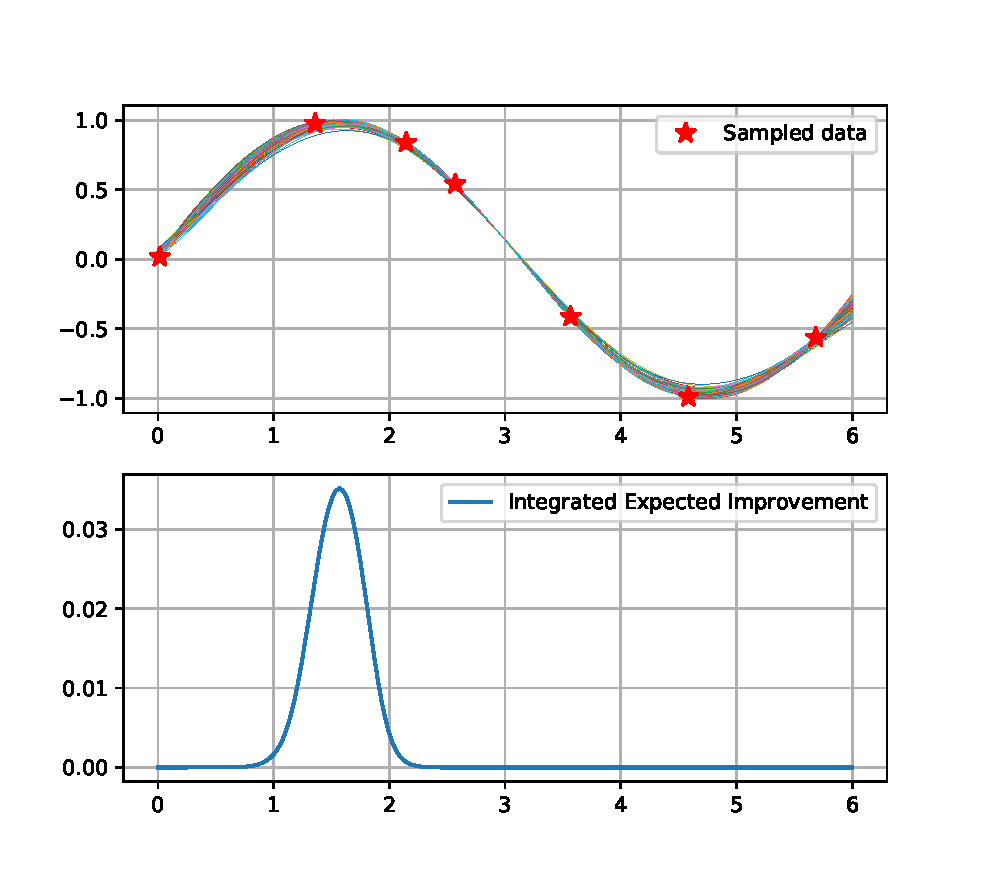
\includegraphics[scale=0.4]{../figures/chapter3/integratedacq}
		\end{figure}
		\end{frame}
		
		\begin{frame}
		\frametitle{Bayesian optimization: optimizing acquisitions}
		We have assumed that the acquisition function is easily optimized. This is not necessarily the case:
		
		\begin{itemize}
		\item It is often multimodal.
		\item Or non-convex.
		\item Furthermore theoretical convergence is guaranteed when finding true maximum $\boldsymbol{x}^{*}$.
		\end{itemize}
		
		One may be thinking that we have switched optimization problems! ($f$ by $\alpha$). However, $\alpha$ 			is very cheap to compute.\\
		\begin{itemize}
		\item In practice $\alpha$ is optimized using multi-start quasi-Newton methods (e.g. L-BFGS-B) or 					evolutionary approaches (CMA-ES).
		\end{itemize}
		\end{frame}
		
		\begin{frame}
		\frametitle{Bayesian optimization: Other surrogates}
		\begin{itemize}
		\item Random Forests: empirical estimate of variance provided by predictions of trees.
		\item Gradient Boosting Machines: using quantile regression for variance estimate.
		\item Sparse pseudo-input GPs
		\item Student-t Processes
		\item ...
		\end{itemize}
		
		\begin{block}{Student-t Process example}
		\begin{equation}
		\boldsymbol{f}^*|\boldsymbol{f} \sim \mathcal{T}\left(\nu + n, \boldsymbol{\phi}_2, \dfrac{\nu + 				\beta_1 - 2}{\nu + n - 2} \tilde{K}_{**} \right)
		\end{equation}
		\end{block}
		\end{frame}
		
		\begin{frame}
			\frametitle{Experiments}
			The aim is to demonstrate that Bayesian Optimization works in real hyperparameter optimization problems.
			\begin{itemize}
				\item Mid-sized supervised learning problems. Both regression and classification considered.
				\item Two examples explained in detail: datasets retrieved from computational chemistry problems.
				\item Other examples drawn from other areas, such as medicine. Available from other sources (UCI ML repository).
			\end{itemize}
		\end{frame}
		
		
		\begin{frame}
		\frametitle{Experiments: benchmarking rules}
		Loss functions used:
		\begin{block}{Binary classification}
		Logarithmic loss:
		\begin{equation}
		\mathcal{L}(\boldsymbol{y}, \boldsymbol{\hat{y}}) = -\dfrac{1}{n} \sum_i \left(y_i \log(\hat{y_i}) + 			(1 - y_i)\log(1-\hat{y_i})\right)
		\end{equation}
		\end{block}
		
		\begin{block}{Regression}
		Mean Squared Error (MSE)
		\begin{equation}
		\mathcal{L}(\boldsymbol{y}, \boldsymbol{\hat{y}}) = \dfrac{1}{n} \sum_i \left(y_i - \hat{y_i}\right)^2
		\end{equation}
		\end{block}
		\end{frame}
		
		\begin{frame}
		\frametitle{Experiments: benchmarking rules}
		\begin{itemize}
		\item Shuffled $k=5$ fold cross-validation scheme for loss evaluation.
		\item Features scaled: zero mean, unit variance.
		\item $n=50$ ($+3$ to account GP fitting) total function evaluations.
		\item Gaussian Process surrogate, with squared exponential covariance function.
		\end{itemize}
		\end{frame}
		
		\begin{frame}
		\frametitle{Experiments: benchmarking rules}
		\begin{itemize}
		\item Type II ML estimation of all hyperparameters at each stage ($l$, $\sigma_n^2$, $\sigma_f^2$).
		\item Expected Improvement and GP-UCB ($\beta = 0.5$, $\beta = 1.5$) acquisitions.
		\item Machine-learning models used: Support Vector Machines, K-Nearest-Neighbours, Gradient Boosting 			Machines and One-Hidden Layer Neural Networks.
		\item Random search is considered as baseline for all experiments.
		\end{itemize}
		\end{frame}
		
		
		\begin{frame}
		\frametitle{Experiments: benchmarking rules}
		\begin{table}[]
		\centering
		\caption{SVM parameters.}
		\label{svmparam}
		\begin{tabular}{@{}lll@{}}
		\toprule
		\textbf{Parameter} & \textbf{Type}                      & \textbf{Bounds}               \\ \midrule
		$C$                & $\mathbb{R}^+$ & $\left[ 10^{-5}, 10^{5} \right]$ (log-scaled) \\
		$\gamma$           & $\mathbb{R}^+$ & $\left[10^{-5}, 10^{5} \right]$  (log-scaled)       \\ 					\bottomrule
		\end{tabular}
		\end{table}
		
		\begin{table}[]
		\centering
		\caption{KNN parameters.}
		\label{knnparams}
		\begin{tabular}{@{}lll@{}}
		\toprule
		\textbf{Parameter} & \textbf{Type} & \textbf{Bounds}                           \\ \midrule
		$k$                & Integer       & $\left\lbrace 10, \dots,50 \right\rbrace$
		\end{tabular}
		\end{table}
		\end{frame}
		
		\begin{frame}
		\frametitle{Experiments: benchmarking rules}
		\begin{table}[]
		\centering
		\caption{GBM parameters.}
		\label{gbmparam}
		\begin{tabular}{@{}lll@{}}
		\toprule
		\textbf{Parameter}             & \textbf{Type}  & \textbf{Bounds}                          \\ \midrule
	\texttt{learning\_rate}      & $\mathbb{R}^+$ & $\left[10^{-5}, 10^{-2}\right]$                         \\
	\texttt{n\_estimators}       & Integer        & $\left\lbrace 10,\dots, 100 \right\rbrace$ \\
	\texttt{max\_depth}          & Integer        & $\left\lbrace 2, \dots, 100 \right\rbrace$ \\
	\texttt{min\_samples\_split}  & Integer        & $\left\lbrace 2, \dots, 100 \right\rbrace$
	\end{tabular}
	\end{table}

\begin{table}[]
\centering
\caption{MLP parameters.}
\label{mlpparam}
\begin{tabular}{lll}
\hline
\textbf{Parameter}             & \textbf{Type}    & \textbf{Bounds}       \\ \hline
\texttt{hidden\_layer\_size} & Integer          & $\left[5, 50\right]$  \\
\texttt{alpha}               & $\mathbb{R}^{+}$ & $\left[0, 0.9\right]$
\end{tabular}
\end{table}

	
		\end{frame}
		
\begin{frame}
	\frametitle{Experiments: Binding affinity prediction dataset}

\begin{itemize}
\item Problem is to predict some binding/inhibition constant between a protein and a ligand ($K_d, K_i$). Target variable is defined as $y = -\log_{10}K$
\end{itemize}			

\begin{figure}
\includegraphics[width=0.6\textwidth]{../figures/chapter4/docking}
\caption{Illustration of the protein-ligand binding scenario.}	
\end{figure}
\end{frame}

\begin{frame}
\frametitle{Experiments: Binding affinity prediction dataset}
\begin{block}{Set of features used}
Pair of atom-type counts from protein and ligand in the binding site.
\begin{align*}
\left\lbrace P_j \right\rbrace_{j=1}^9 = \left\lbrace C, N, O, F, P, S, Cl, Br, I \right\rbrace \\
\left\lbrace L_i \right\rbrace_{i=1}^9 = \left\lbrace C, N, O, F, P, S, Cl, Br, I \right\rbrace
\end{align*}
\begin{equation}
\boldsymbol{x}\left(Z(P_j), Z(L_i)\right) = \sum_{k=1}^{P_j}\sum_{l=1}^{L_i}\Theta (d_{\mathrm{cutoff}} - d_{kl})
\end{equation}
\end{block}

\begin{block}{Data}
\begin{itemize}
\item PDBbind v.2015 database of affinity and kinetic biological data.
\item  A refined set of $n=3623$ of protein-ligand pairs for training, and another $m=195$ structurally diverse for testing.
\end{itemize}
\end{block}
\end{frame}

\begin{frame}
\frametitle{Experiments: Binding affinity prediction dataset}
\begin{figure}[ht]
  \centering
  \caption{Benchmarking results for the binding affinity dataset (1/2).}
  \begin{subfigure}[t]{0.5\textwidth}
  	\caption{SVM}
    \centering\includegraphics[width=\textwidth]{../figures/chapter4/aff/svm}
  \end{subfigure}%
  \begin{subfigure}[t]{0.5\textwidth}
    \caption{KNN}
    \centering\includegraphics[width=\textwidth]{../figures/chapter4/aff/knn}
  \end{subfigure}
  \label{fig:aff}
\end{figure}

\end{frame}

\begin{frame}
\frametitle{Experiments: Binding affinity prediction dataset}
\begin{figure}[ht]
  \centering
  \caption{Benchmarking results for the binding affinity dataset (2/2).}
    \begin{subfigure}[t]{0.5\textwidth}
    \caption{MLP}
    \centering\includegraphics[width=\textwidth]{../figures/chapter4/aff/mlp}
  \end{subfigure}%
    \begin{subfigure}[t]{0.5\textwidth}
    \caption{GBM}
    \centering\includegraphics[width=\textwidth]{../figures/chapter4/aff/gbm}
  \end{subfigure}
  \label{fig:aff2}
\end{figure}
\end{frame}

\begin{frame}
\frametitle{Experiments: Protein-protein interface prediction}
\begin{itemize}
\item Predict whether a particular residue is in contact with a chain of another protein.
\item Interfaces are \textbf{not} considered target-specific.
\begin{figure}
\includegraphics[width=0.6\textwidth]{../figures/chapter4/interface}
\caption{An interface between two chains of a dimer. Residues considered interficial are marked in blue.}	
\end{figure}
\end{itemize}
\end{frame}


\begin{frame}
\frametitle{Experiments: Protein-protein interface prediction}
\begin{block}{Features used}
Descriptors resemble those detailed in (Jim\'enez \textit{et al}. 2017). Average pharmacophoric-like features computed in a particular neighbourhood (20\AA$^3$) of a residue.
\end{block}

\begin{block}{Data}
PIFACE database of clustered protein interface. Over 22k structurally unique interfaces extracted from the Protein Data Bank.
\end{block}
\end{frame}

\begin{frame}
\frametitle{Experiments: Protein-protein interface prediction}
\begin{figure}[ht]
  \centering
  \caption{Benchmarking results for the protein-protein interface dataset (1/2).}
  \begin{subfigure}[t]{0.5\textwidth}
  	\caption{SVM}
    \centering\includegraphics[width=\textwidth]{../figures/chapter4/pinter/svm}
  \end{subfigure}%
  \begin{subfigure}[t]{0.5\textwidth}
    \caption{KNN}
    \centering\includegraphics[width=\textwidth]{../figures/chapter4/pinter/knn}
  \end{subfigure}
  \label{fig:aff}
\end{figure}
\end{frame}

\begin{frame}
\frametitle{Experiments: Protein-protein interface prediction}
\begin{figure}[ht]
  \centering
  \caption{Benchmarking results for the protein-protein interface dataset (2/2).}
  \begin{subfigure}[t]{0.5\textwidth}
  	\caption{MLP}
    \centering\includegraphics[width=\textwidth]{../figures/chapter4/pinter/mlp}
  \end{subfigure}%
  \begin{subfigure}[t]{0.5\textwidth}
    \caption{GBM}
    \centering\includegraphics[width=\textwidth]{../figures/chapter4/pinter/gbm}
  \end{subfigure}
  \label{fig:aff}
\end{figure}
\end{frame}

\begin{frame}
\frametitle{Experiments: other datasets}
\begin{figure}[ht]
  \centering
  \caption{Benchmarking results for the LSVT Voice Rehabilitation dataset.}
  \begin{subfigure}[t]{0.5\textwidth}
  	\caption{SVM}
    \centering\includegraphics[width=\textwidth]{../figures/chapter4/lsvt/svm}
  \end{subfigure}%
  \begin{subfigure}[t]{0.5\textwidth}
    \caption{KNN}
    \centering\includegraphics[width=\textwidth]{../figures/chapter4/lsvt/knn}
  \end{subfigure}
  \label{fig:breastcancer}
\end{figure}
\end{frame}

\begin{frame}
\frametitle{Experiments: other datasets}
\begin{figure}[ht]
  \centering
  \caption{Benchmarking results for the LSVT Voice Rehabilitation dataset.}
  \begin{subfigure}[t]{0.5\textwidth}
  	\caption{MLP}
    \centering\includegraphics[width=\textwidth]{../figures/chapter4/lsvt/mlp}
  \end{subfigure}%
  \begin{subfigure}[t]{0.5\textwidth}
    \caption{GBM}
    \centering\includegraphics[width=\textwidth]{../figures/chapter4/lsvt/gbm}
  \end{subfigure}
  \label{fig:breastcancer}
\end{figure}
\end{frame}

\begin{frame}
\frametitle{Experiments: other datasets}
\begin{figure}[ht]
  \centering
  \caption{Benchmarking results for the Parkinson's dataset.}
  \begin{subfigure}[t]{0.5\textwidth}
  	\caption{SVM}
    \centering\includegraphics[width=\textwidth]{../figures/chapter4/parkinson/svm}
  \end{subfigure}%
  \label{fig:park}
\end{figure}
\end{frame}

\begin{frame}
\frametitle{Experiments: other datasets}
\begin{figure}[ht]
  \centering
  \caption{Benchmarking results for the Parkinson's dataset.}
  \begin{subfigure}[t]{0.5\textwidth}
  	\caption{MLP}
    \centering\includegraphics[width=\textwidth]{../figures/chapter4/parkinson/mlp}
  \end{subfigure}%
  \begin{subfigure}[t]{0.5\textwidth}
    \caption{GBM}
    \centering\includegraphics[width=\textwidth]{../figures/chapter4/parkinson/gbm}
  \end{subfigure}
  \label{fig:park}
\end{figure}
\end{frame}

\begin{frame}
\frametitle{Experiments: other datasets}
\begin{figure}[ht]
  \centering
  \caption{Benchmarking results for the Breast cancer dataset.}
  \begin{subfigure}[t]{0.5\textwidth}
  	\caption{SVM}
    \centering\includegraphics[width=\textwidth]{../figures/chapter4/breast/svm}
  \end{subfigure}%
  \begin{subfigure}[t]{0.5\textwidth}
    \caption{KNN}
    \centering\includegraphics[width=\textwidth]{../figures/chapter4/breast/knn}
  \end{subfigure}
  \label{fig:breastcancer}
\end{figure}
\end{frame}

\begin{frame}
\frametitle{Experiments: other datasets}
\begin{figure}[ht]
  \centering
  \caption{Benchmarking results for the Breast cancer dataset.}
  \begin{subfigure}[t]{0.5\textwidth}
  	\caption{MLP}
    \centering\includegraphics[width=\textwidth]{../figures/chapter4/breast/mlp}
  \end{subfigure}%
  \begin{subfigure}[t]{0.5\textwidth}
    \caption{GBM}
    \centering\includegraphics[width=\textwidth]{../figures/chapter4/breast/gbm}
  \end{subfigure}
  \label{fig:breastcancer}
\end{figure}
\end{frame}

\begin{frame}
\frametitle{pyGPGO: Bayesian Optimization for Python}
There are many possible choices in the Bayesian Optimization framework:
\begin{itemize}
\item Choice of surrogate model.
\item Covariance function to use
\item Acquisition behaviour
\item Hyperparameter treatment
\end{itemize}
They naturally motivate a modular design. Most of the available software focuses on a particular
implementation of the Bayesian optimization algorithm.\\

pyGPGO is a package I wrote to cover as many of these scenarios as possible.
\end{frame}

\begin{frame}
\frametitle{pyGPGO: features}
pyGPGO features:
\begin{itemize}
\item A completely modular and customizable design. Easy to setup and minimal dependencies.
\item A wide range of surrogate models: Gaussian Processes, Student-t Processes, Random Forests, Extra Random Forests and Gradient Boosting Machines.
\item Most of the usual covariance functions, as well as its derivatives: squared exponential, Mat\'ern, $\gamma$-exponential, rational quadratic, exponential sine, and dot product.
\item Many acquisition function behaviours: probability of improvement, expected improvement, upper confidence bound and entropy-based, as well as their integrated versions.
\item Type II Maximum-Likelihood of covariance function hyperparameters.
\item MCMC sampling for full-Bayesian treatment of hyperparameters (via \texttt{pyMC3}).
\end{itemize}
\end{frame}

\begin{frame}[fragile]
\frametitle{pyGPGO: a simple example}
\begin{minted}[mathescape,
               linenos,
               fontsize=\footnotesize ,
               numbersep=5pt,
               gobble=0,
               frame=lines,
               framesep=2mm,
               python3 = true]{python}
import numpy as np
from pyGPGO.covfunc import matern32
from pyGPGO.acquisition import Acquisition
from pyGPGO.surrogates.GaussianProcess import GaussianProcess
from pyGPGO.GPGO import GPGO


def f(x, y):
    # Franke's function (https://www.mathworks.com/help/curvefit/franke.html)
    one = 0.75 * np.exp(-(9 * x - 2) ** 2 / 4 - (9 * y - 2) ** 2 / 4)
    two = 0.75 * np.exp(-(9 * x + 1) ** 2/ 49 - (9 * y + 1) / 10)
    three = 0.5 * np.exp(-(9 * x - 7) ** 2 / 4 - (9 * y -3) ** 2 / 4)
    four = 0.25 * np.exp(-(9 * x - 4) ** 2 - (9 * y - 7) ** 2)
    return one + two + three - four
\end{minted}
\end{frame}

\begin{frame}[fragile]
\frametitle{pyGPGO: a simple example}
\begin{minted}[mathescape,
               linenos,
               fontsize=\footnotesize ,
               numbersep=5pt,
               gobble=0,
               frame=lines,
               framesep=2mm,
               python3 = true]{python}
cov = matern32()
gp = GaussianProcess(cov)
acq = Acquisition(mode='ExpectedImprovement')
param = {'x': ('cont', [0, 1]),
         'y': ('cont', [0, 1])}

np.random.seed(1337)
gpgo = GPGO(gp, acq, f, param)
gpgo.run(max_iter=10)
gpgo.getResult()
\end{minted}
\end{frame}

\begin{frame}[fragile]
\frametitle{pyGPGO: optimizing SVM hyperparameters}
\begin{minted}[mathescape,
               linenos,
               fontsize=\footnotesize ,
               numbersep=5pt,
               gobble=0,
               frame=lines,
               framesep=2mm,
               python3 = true]{python}

import numpy as np
from sklearn.datasets import make_moons
from sklearn.svm import SVC
from sklearn.model_selection import cross_val_score


from pyGPGO.GPGO import GPGO
from pyGPGO.surrogates.GaussianProcess import GaussianProcess
from pyGPGO.acquisition import Acquisition
from pyGPGO.covfunc import squaredExponential


def evaluateModel(C, gamma):
    clf = SVC(C=10**C, gamma=10**gamma)
    return np.average(cross_val_score(clf, X, y))
               
\end{minted}
\end{frame}

\begin{frame}[fragile]
\frametitle{pyGPGO: optimizing SVM hyperparameters}
\begin{minted}[mathescape,
               linenos,
               fontsize=\footnotesize ,
               numbersep=5pt,
               gobble=0,
               frame=lines,
               framesep=2mm,
               python3 = true]{python}
               
X, y = make_moons(n_samples = 200, noise = 0.3)
    
sexp = squaredExponential()
gp = GaussianProcess(sexp, optimize = True, usegrads = True)
acq = Acquisition(mode = 'UCB', beta = 1.5)

params = {'C':      ('cont', (-4, 5)),
          'gamma':  ('cont', (-4, 5))}

gpgo = GPGO(gp, acq, evaluateModel, params)
gpgo.run(max_iter = 50)
gpgo.getResult()
\end{minted}
\end{frame}

\begin{frame}
\frametitle{pyGPGO: Bayesian Optimization for Python}
\begin{columns}
\column{0.7\linewidth}
\centering
\begin{itemize}
\item The software is MIT licensed and can be downloaded from its GitHub repository @ \textcolor{blue}{\url{https://github.com/hawk31/pyGPGO}}
\item Extensive documentation can be found in ReadTheDocs. \textcolor{blue}{\url{pygpgo.readthedocs.io/en/latest}}
\item Anyone can contribute to the project! (Implement new features, report bugs, improve docs...)
\item All benchmarking, examples and thesis code is also available. 
\end{itemize}
\column{0.58\linewidth}
\begin{figure}

\includegraphics[width=0.4\textwidth]{figures/github}
\end{figure}
\end{columns}
\end{frame}

\begin{frame}
\frametitle{pyGPGO in numbers}
\begin{figure}
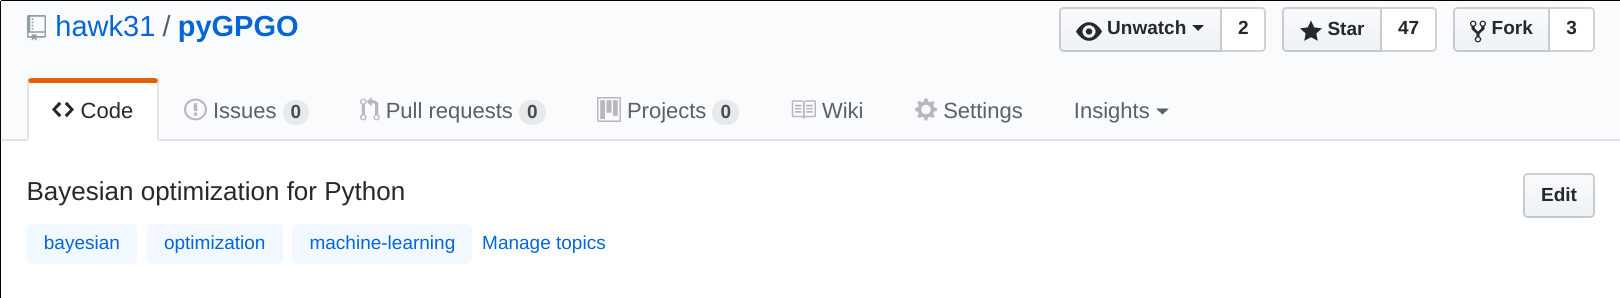
\includegraphics[width=\textwidth]{figures/pygpgo_git}\\
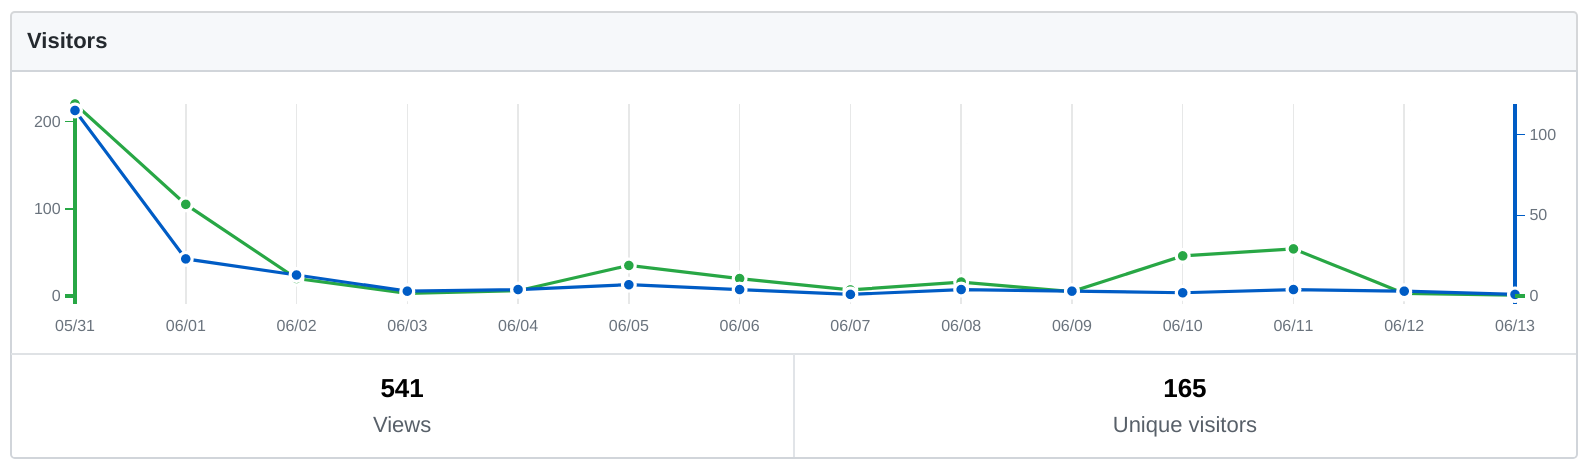
\includegraphics[width=\textwidth]{figures/visits}\\
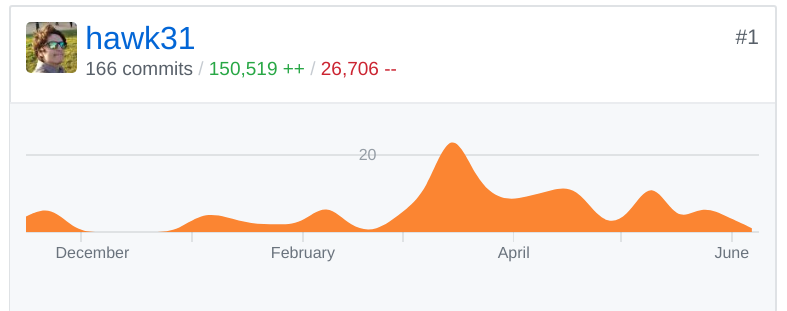
\includegraphics[scale=0.3]{figures/commits}
\end{figure}
\end{frame}

\begin{frame}
\frametitle{pyGPGO: Future work}
Like any other piece of software, there is always stuff to do!
\begin{itemize}
\item Constrained optimization. $P\left(\mathcal{C}(\boldsymbol{x})\right) \geq 1 - \delta$
\item Better support for non-stationary covariance functions.
\item GPU support for non-MCMC samplers (BBVI).
\item A parallel interface for experiment running.
\item More acquisitions, surrogates...
\end{itemize}
\end{frame}

\begin{frame}[plain,c]
\usebeamerfont*{frametitle}
\begin{columns}
\column{0.5\linewidth}
\Huge Thank you\\
\Large {Q\&A time!} 
\column{0.5\linewidth}
\normalsize
{Acknowledgements to :
\begin{itemize}
\item Josep Ginebra
\item V\'ictor Peña
\end{itemize}
}
My lab co-workers @ \textcolor{red}{UPF} for letting me spend time on this project!
\begin{itemize}
\item Gianni de Fabritiis
\item Stefan Doerr
\item Gerard Mart\'inez
\item Miha \v{S}kali\v{c}
\item Pablo Herrera
\item Jo\~ao Damas
\end{itemize}
\end{columns}
\end{frame}
			
			

\end{document}